\documentclass[12pt,a4paper]{article}

\usepackage{fontspec}
\usepackage{amsmath,amssymb,mathtools}
\usepackage{geometry}
\usepackage{enumitem}
\usepackage{booktabs}
\usepackage{array}
\usepackage{xcolor}
\usepackage{tikz}
\usepackage{listings}
\usepackage{fancyhdr}
\usepackage{hyperref}
\usepackage{microtype}

\setmainfont{Times New Roman}[
  Path=/System/Library/Fonts/Supplemental/,
  UprightFont=Times New Roman.ttf,
  BoldFont=Times New Roman Bold.ttf,
  ItalicFont=Times New Roman Italic.ttf,
  BoldItalicFont=Times New Roman Bold Italic.ttf
]
\setsansfont{Arial}[
  Path=/System/Library/Fonts/Supplemental/,
  UprightFont=Arial.ttf,
  BoldFont=Arial Bold.ttf,
  ItalicFont=Arial Italic.ttf,
  BoldItalicFont=Arial Bold Italic.ttf
]
\setmonofont{Menlo}[Path=/System/Library/Fonts/,UprightFont=Menlo.ttc,Scale=0.84]

\geometry{top=2.2cm,bottom=2.2cm,left=2.5cm,right=2.5cm}
\setlength{\parindent}{0pt}
\setlength{\parskip}{0.55em}
\setlist[itemize]{leftmargin=1.6em,itemsep=0.25em,topsep=0.3em}
\setlist[enumerate]{leftmargin=1.8em,itemsep=0.3em,topsep=0.3em}

\definecolor{navy}{HTML}{17365D}
\definecolor{lightblue}{HTML}{EAF2F8}
\definecolor{darkgray}{HTML}{444444}
\definecolor{codebg}{HTML}{F5F7F9}

\hypersetup{
  colorlinks=true,
  linkcolor=navy,
  urlcolor=navy,
  pdftitle={Homework 1 - Blockchain},
  pdfauthor={Nhom 12 - R2R}
}

\pagestyle{fancy}
\fancyhf{}
\setlength{\headheight}{14pt}
\fancyhead[L]{\small 20261A - Blockchain}
\fancyhead[R]{\small Nhóm 12 - R2R}
\fancyfoot[C]{\thepage}
\renewcommand{\headrulewidth}{0.4pt}

\lstdefinestyle{bitcoin}{
  basicstyle=\ttfamily\small,
  backgroundcolor=\color{codebg},
  frame=single,
  rulecolor=\color{darkgray!35},
  framesep=7pt,
  aboveskip=0.8em,
  belowskip=0.8em,
  columns=fullflexible,
  keepspaces=true
}

\newcommand{\problem}[2]{%
  \clearpage
  \section*{\color{navy}Bài #1. #2}
  \addcontentsline{toc}{section}{Bài #1. #2}
}

\newenvironment{summarybox}
  {\begin{quote}\small\color{darkgray}\textbf{Tóm tắt đề.}\;}
  {\end{quote}}

\newcommand{\solution}{\subsection*{Bài làm}}
\newcommand{\concat}{\mathbin{\|}}
\renewcommand{\contentsname}{Mục lục}

\begin{document}

\hypersetup{pageanchor=false}
\begin{titlepage}
  \centering
  {\large\sffamily HỌC PHẦN 20261A - BLOCKCHAIN\par}
  \vspace{1.8cm}
  {\color{navy}\rule{0.88\textwidth}{1.2pt}\par}
  \vspace{0.65cm}
  {\Huge\bfseries BÀI TẬP VỀ NHÀ SỐ 1\par}
  \vspace{0.35cm}
  {\Large Mật mã học, Merkle tree và Bitcoin\par}
  \vspace{0.65cm}
  {\color{navy}\rule{0.88\textwidth}{1.2pt}\par}

  \vfill

  \begin{tabular}{>{\bfseries}l l l}
    \toprule
    Nhóm & Họ và tên & Mã học viên \\
    \midrule
    12 - R2R & Trần Mạnh Đạt & 20252607M \\
              & Trần Hoàng Sơn & 20252606M \\
              & Nguyễn Đức Hoàng & 20252603M \\
    \bottomrule
  \end{tabular}

  \vfill
  {\large Ngày 14 tháng 10 năm 2026\par}
  \vspace{0.8cm}
  {\small Tài liệu gốc: Stanford CS251 - Assignment \#1 (Fall 2023)\par}
\end{titlepage}

\hypersetup{pageanchor=true}
\pagenumbering{roman}
\tableofcontents
\clearpage
\pagenumbering{arabic}

\problem{1}{Hàm proof of work không an toàn}

\begin{summarybox}
Xét $H(x,y)=\operatorname{SHA256}(x\oplus y)$ và độ khó $D$ đã biết trước.
Chứng minh kẻ tấn công có thể chuẩn bị phần lớn công việc trước khi thử thách
$x$ được công bố, rồi tìm nghiệm $y$ gần như tức thời.
\end{summarybox}

\solution

Kẻ tấn công chia quá trình thành hai giai đoạn.

\subsection*{Giai đoạn 1: tiền tính toán ngoại tuyến}

Trước khi biết $x$, kẻ tấn công chọn các chuỗi
$z\in\{0,1\}^{m}$ và thử cho đến khi tìm được $z^*$ thỏa
\[
  \operatorname{SHA256}(z^*) < \frac{2^{256}}{D}.
\]

Nếu đầu ra SHA256 phân bố đều trên $\{0,1,\ldots,2^{256}-1\}$, xác suất
một lần thử thành công xấp xỉ
\[
  p=\frac{2^{256}/D}{2^{256}}=\frac{1}{D}.
\]
Do đó số lần băm kỳ vọng để tìm được $z^*$ là
\[
  \mathbb{E}[N]=\frac{1}{p}=D.
\]
Kẻ tấn công lưu $z^*$ lại. Chi phí $D$ phép băm đã được trả trước và không
phụ thuộc vào thử thách cụ thể sẽ xuất hiện sau đó.

\subsection*{Giai đoạn 2: giải trực tuyến}

Ngay khi $x$ được công bố, đặt
\[
  y=x\oplus z^*.
\]
Khi đó
\begin{align*}
  H(x,y)
    &=\operatorname{SHA256}(x\oplus y)\\
    &=\operatorname{SHA256}\bigl(x\oplus(x\oplus z^*)\bigr)\\
    &=\operatorname{SHA256}\bigl((x\oplus x)\oplus z^*\bigr)\\
    &=\operatorname{SHA256}(z^*)\\
    &<\frac{2^{256}}{D}.
\end{align*}

Chi phí sau khi nhận $x$ chỉ là một phép XOR trên $m$ bit; không cần gọi lại
SHA256. Vì công việc tính toán không bị ràng buộc với thử thách mới $x$, hàm
$H$ không an toàn để dùng làm proof of work.

\problem{2}{Cây Merkle \texorpdfstring{$k$}{k}-phân}

\begin{summarybox}
Mở rộng Merkle tree nhị phân thành cây mà mỗi nút trong có tối đa $k$ nút con.
Xây commitment tam phân cho $S=(T_1,\ldots,T_9)$, chứng minh $T_4\in S$, tính
độ dài bằng chứng tổng quát và so sánh cây nhị phân với cây tam phân.
\end{summarybox}

\solution

Ký hiệu $h$ là hàm băm, $\concat$ là phép nối chuỗi và $L_i=h(T_i)$.

\subsection*{a) Cây tam phân với chín phần tử}

Vì $9=3^2$, cây có đúng hai tầng phía trên các lá.

\begin{figure}[h]
\centering
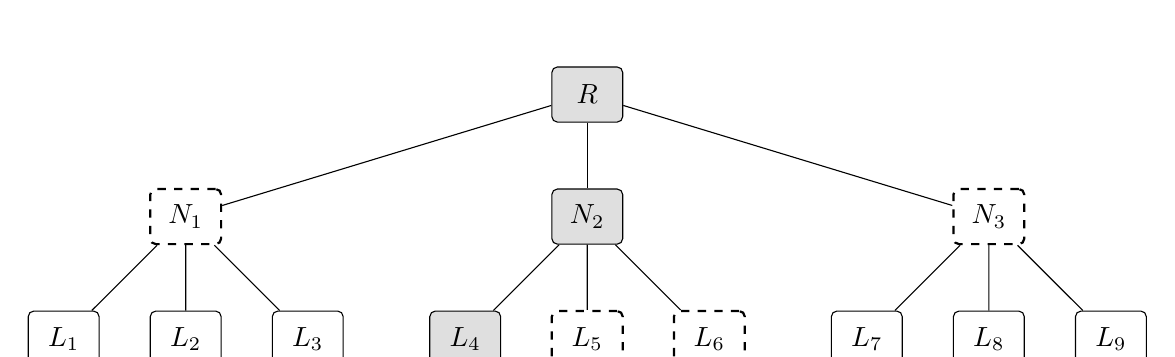
\begin{tikzpicture}[
  level distance=1.55cm,
  level 1/.style={sibling distance=5.1cm},
  level 2/.style={sibling distance=1.55cm},
  every node/.style={draw,rounded corners=2pt,minimum width=9mm,minimum height=7mm},
  path/.style={fill=gray!25},
  proof/.style={dashed,thick}
]
\node[path] {$R$}
  child {node[proof] {$N_1$}
    child {node {$L_1$}}
    child {node {$L_2$}}
    child {node {$L_3$}}
  }
  child {node[path] {$N_2$}
    child {node[path] {$L_4$}}
    child {node[proof] {$L_5$}}
    child {node[proof] {$L_6$}}
  }
  child {node[proof] {$N_3$}
    child {node {$L_7$}}
    child {node {$L_8$}}
    child {node {$L_9$}}
  };
\end{tikzpicture}
\caption{Đường tô xám đi từ $L_4$ lên gốc; nút viền đứt thuộc bằng chứng.}
\end{figure}

Alice tính
\begin{align*}
  N_1&=h(L_1\concat L_2\concat L_3), &
  N_2&=h(L_4\concat L_5\concat L_6),\\
  N_3&=h(L_7\concat L_8\concat L_9), &
  R&=h(N_1\concat N_2\concat N_3).
\end{align*}
Alice công bố $R$ làm commitment của danh sách $S$.

Để chứng minh $T_4\in S$, Alice gửi $T_4$, chỉ số $i=4$ và
\[
  \pi=(L_5,L_6,N_1,N_3),
\]
tức bốn giá trị băm. Bob tính
\[
  L_4=h(T_4),\qquad
  N_2=h(L_4\concat L_5\concat L_6),\qquad
  R'=h(N_1\concat N_2\concat N_3).
\]
Nếu $R'=R$, Bob chấp nhận. Chỉ số $i=4$ cho Bob biết đúng thứ tự ghép các
giá trị. Khả năng Alice thay $T_4$ bằng một giá trị khác mà vẫn cho cùng gốc
sẽ dẫn đến một va chạm của $h$.

\subsection*{b) Độ dài bằng chứng}

Cây có độ sâu tối đa
\[
  d=\left\lceil\log_k n\right\rceil.
\]
Ở mỗi tầng, verifier cần nhiều nhất $k-1$ hash anh em. Do đó
\[
  \boxed{|\pi|\le (k-1)\left\lceil\log_k n\right\rceil}
\]
giá trị băm. Nếu tầng cuối không đủ $k$ con thì bằng chứng thực tế có thể ngắn
hơn; đây là cận trên khi cấu trúc cây hoặc quy tắc padding đã được thống nhất.

\subsection*{c) Nhị phân hay tam phân?}

Với $n$ lớn và bỏ qua phép làm tròn,
\[
  |\pi_k|\approx(k-1)\log_k n
  =\frac{k-1}{\ln k}\ln n.
\]
Hai trường hợp cần so sánh là
\[
  |\pi_2|\approx\frac{1}{\ln2}\ln n\approx1.443\ln n,
  \qquad
  |\pi_3|\approx\frac{2}{\ln3}\ln n\approx1.820\ln n.
\]
Vì vậy nên dùng cây nhị phân. Bằng chứng tam phân dài hơn khoảng
$1.820/1.443-1\approx26.2\%$. Việc tăng $k$ làm cây thấp đi theo $\ln k$,
nhưng số hash anh em ở mỗi tầng lại tăng tuyến tính theo $k-1$.

\problem{3}{Bitcoin Script và mật khẩu}

\begin{summarybox}
Một UTXO dùng hashlock mật khẩu với script được in trong đề là
\texttt{OP\_SHA256 <eb27...f69b> OP\_EQUAL}. Viết dữ liệu mở khóa và phân tích
rủi ro với mật khẩu ngắn cũng như passphrase mạnh.
\end{summarybox}

\solution

\subsection*{Lỗi độ dài trong đề Fall 2023}

\texttt{OP\_SHA256} luôn trả về digest 32 byte. Hằng
\texttt{eb271cbcc2340d0b0e6212903e29f22e578ff69b} có 40 ký tự hex, tức 20
byte. Hai byte-string khác độ dài không thể bằng nhau, nên script đúng nguyên
văn là \textbf{không thể tiêu}, ngay cả khi biết mật khẩu $P$.

Ý đồ của bài là một hashlock. Có thể sửa bằng cách đổi opcode thành
\texttt{OP\_SHA1} để phù hợp với digest 20 byte, hoặc giữ
\texttt{OP\_SHA256} và thay hằng bằng digest SHA256 32 byte của $P$. Các câu
trả lời sau dùng phiên bản đã sửa.

\subsection*{a) ScriptSig}

\begin{lstlisting}[style=bitcoin]
<P>
\end{lstlisting}

ScriptSig chỉ đẩy byte-string của mật khẩu lên stack. ScriptPubKey băm nó rồi
so sánh với digest đã cam kết; không có public key hoặc chữ ký số.

\subsection*{b) Mật khẩu sáu ký tự}

Digest đã công khai trong output. Kẻ tấn công có thể duyệt ngoại tuyến toàn bộ
không gian mật khẩu sáu ký tự, băm từng ứng viên và so sánh với digest. Khi tìm
được $P$, họ tự tạo giao dịch tiêu UTXO về địa chỉ của mình. SHA256 được thiết
kế để tính nhanh nên không thay thế một hàm password hashing có salt và có chi
phí tính toán cao.

\subsection*{c) Passphrase mạnh 30 ký tự}

Passphrase mạnh ngăn được vét cạn trước khi Alice tiêu coin, nhưng hashlock đơn
lẻ vẫn không an toàn:
\begin{enumerate}[nosep]
  \item Alice phát giao dịch; $P$ xuất hiện công khai trong ScriptSig.
  \item Nút mạng hoặc miner đọc $P$ từ mempool.
  \item Họ tạo giao dịch cạnh tranh dùng cùng $P$, chuyển coin về địa chỉ của
        họ và có thể đặt phí cao hơn.
  \item Script không có chữ ký ràng buộc người nhận hoặc nội dung giao dịch,
        nên giao dịch thay thế cũng hợp lệ.
\end{enumerate}
Do đó, cần kết hợp hashlock với điều kiện chữ ký như \texttt{OP\_CHECKSIG}.

\problem{4}{BitcoinLotto}

\begin{summarybox}
Thiết kế jackpot Bitcoin sao cho vé thắng không thể nhận giải trước cuối tuần,
đồng thời jackpot chưa nhận của các tuần trước có thể chuyển cho người thắng
tuần sau mà không trao thêm quyền biển thủ cho ban tổ chức.
\end{summarybox}

\solution

Gọi $(sk_i,PK_i)$ là cặp khóa của vé trúng tuần $i$. Nhà in đáng tin cậy đặt
$sk_i$ dưới lớp cào của đúng một vé thắng và không lưu bản sao.

\subsection*{a) Chỉ cho nhận giải vào cuối tuần}

Khóa output bằng \texttt{OP\_CHECKLOCKTIMEVERIFY} (CLTV):
\begin{lstlisting}[style=bitcoin]
<T_end> OP_CHECKLOCKTIMEVERIFY OP_DROP <PK_i> OP_CHECKSIG
\end{lstlisting}

$T_{\mathrm{end}}$ là block height hoặc Unix timestamp ứng với cuối tuần. Giao
dịch nhận giải phải thỏa:
\begin{itemize}
  \item \texttt{nLockTime >= T\_end} và cùng kiểu height/time với
        $T_{\mathrm{end}}$;
  \item \texttt{nSequence} của input khác \texttt{0xffffffff};
  \item chữ ký hợp lệ tạo bởi $sk_i$.
\end{itemize}
Trước $T_{\mathrm{end}}$, CLTV làm script thất bại. Sau thời điểm đó, chỉ người
giữ vé thắng mới tạo được chữ ký hợp lệ.

\subsection*{b) Chuyển jackpot chưa nhận sang tuần sau}

Vì hệ thống chạy đúng 1000 tuần, nhà in sinh trước 1000 cặp khóa và công bố
toàn bộ public key. Jackpot mới của tuần $i$ được khóa theo điều kiện
$1$-of-$(1001-i)$ giữa khóa tuần hiện tại và tất cả khóa các tuần sau:
\begin{lstlisting}[style=bitcoin]
1 <PK_i> <PK_(i+1)> ... <PK_1000> (1001-i) OP_CHECKMULTISIG
\end{lstlisting}

Có thể đặt điều kiện này sau CLTV ở câu a. Nếu jackpot tuần $i$ chưa được
nhận, khóa $sk_{i+1}$ của người thắng tuần sau cũng tiêu được output tuần $i$.
Tổng quát, người thắng tuần $j$ có thể gom mọi UTXO chưa nhận của các tuần
$i\le j$ vào một giao dịch. Ban tổ chức không nắm private key nào, nên không có
thêm cách biển thủ so với mô hình ban đầu; giả thiết nhà in không giữ khóa vẫn
là giả thiết tin cậy cốt lõi.

Đây là thiết kế khái niệm mà bài tập hướng tới. Bitcoin hiện hành giới hạn số
public key trong \texttt{OP\_CHECKMULTISIG} và giới hạn kích thước script, nên
không thể đặt đủ 1000 khóa trong một script thực tế. Một triển khai thật phải
chia rollover thành nhiều giai đoạn, dùng giao dịch ký sẵn hoặc cấu trúc script
hiện đại hơn.

\problem{5}{Lightweight client}

\begin{summarybox}
Bob chỉ giữ block header ở head hiện tại. Xác định dữ liệu Alice phải gửi để
chứng minh giao dịch thanh toán nằm trong một block tổ tiên, rồi tính kích thước
bằng chứng khi block đó cách head $k$ block và mỗi block có $n$ giao dịch.
\end{summarybox}

\solution

Giả sử giao dịch nằm trong block $B_0$, còn block Bob đang giữ là $B_k$:
\[
  B_0 \longleftarrow B_1 \longleftarrow \cdots
  \longleftarrow B_{k-1} \longleftarrow B_k.
\]

\subsection*{a) Dữ liệu Alice phải gửi}

Alice gửi:
\begin{enumerate}
  \item giao dịch thanh toán để Bob kiểm tra output thực sự trả tiền cho mình;
  \item Merkle inclusion proof từ TXID đến Merkle root trong header $B_0$,
        kèm thông tin vị trí trái/phải;
  \item các header $B_0,B_1,\ldots,B_{k-1}$.
\end{enumerate}

Bob băm giao dịch để lấy TXID, dùng Merkle proof tính lại root rồi so sánh với
trường Merkle root của $B_0$. Tiếp theo, Bob băm từng header và kiểm tra hash
của $B_i$ bằng trường previous-block-hash trong $B_{i+1}$. Bước cuối so sánh
hash của $B_{k-1}$ với previous-block-hash trong $B_k$ mà Bob đã tin cậy.

Merkle proof chứng minh giao dịch thuộc $B_0$; chuỗi header chứng minh $B_0$
là tổ tiên của head hiện tại.

\subsection*{b) Kích thước bằng chứng}

Merkle proof nhị phân cho $n$ giao dịch cần
$\lceil\log_2 n\rceil$ hash. Mỗi hash SHA256 dài 32 byte và mỗi Bitcoin block
header dài 80 byte. Bob đã có header head nên Alice cần gửi $k$ header còn lại.
Bỏ qua kích thước giao dịch và vài bit metadata chỉ hướng trái/phải:
\[
  \boxed{S(n,k)=32\left\lceil\log_2 n\right\rceil+80k\ \text{byte}.}
\]

Với $k=6$ và $n=1024=2^{10}$:
\[
  S=32\cdot10+80\cdot6=320+480=\boxed{800\ \text{byte}}.
\]
Nếu tính cả giao dịch thanh toán, cần cộng thêm kích thước serialized
transaction $|tx|$. Con số 800 byte là phần bằng chứng xác thực mà đề cung cấp
đủ dữ kiện để tính.

\clearpage
\section*{Tài liệu kiểm chứng}
\addcontentsline{toc}{section}{Tài liệu kiểm chứng}

\begin{enumerate}
  \item Stanford CS251, \emph{Assignment \#1, Fall 2023}:\\
        \url{https://securitylab.github.io/cs251-fall23/hw/hw1.pdf}
  \item BIP 65, \emph{OP\_CHECKLOCKTIMEVERIFY}:\\
        \url{https://github.com/bitcoin/bips/blob/master/bip-0065.mediawiki}
  \item Bitcoin Developer Reference, \emph{Block Chain}:\\
        \url{https://developer.bitcoin.org/reference/block_chain.html}
  \item Bitcoin Developer Guide, \emph{Simplified Payment Verification}:\\
        \url{https://developer.bitcoin.org/devguide/operating_modes.html}
  \item Bitcoin Developer Reference, \emph{Transactions}:\\
        \url{https://developer.bitcoin.org/reference/transactions.html}
\end{enumerate}

\end{document}
